\section{Methodology}
\label{sec:method}
% ========= object centric =========

We have introduced our method somewhat in the previous section and
justified our design decisions in the light of related literature.  In
this section we present our method for modularizing human
demonstrations of manipulation tasks. Our goal is to acquire a modular
control policy for an object manipulation task from this human
demonstration. To this end, we take a three-step approach:
\begin{enumerate}
\item Human demonstration of a task in several different contexts (Section~\ref{sec:demo}).
%\item Clustering the data to find number of modules needed in the task (subsection ~\ref{sec:cluster}).
\item Extraction and modular decomposition of human control strategies
  for different contexts, abuilding multiple internal models
  (Section~\ref{sec:learn}).
%\item Design a controller based on the learnt multiple model  (subsection ~\ref{controller}).
\item Robot control using the integrated modules to compute motor
  commands (Section~\ref{sec:control}).
\end{enumerate}
Figure~\ref{fig:overview} shows an overview of our framework.

\begin{figure}
  \centering
   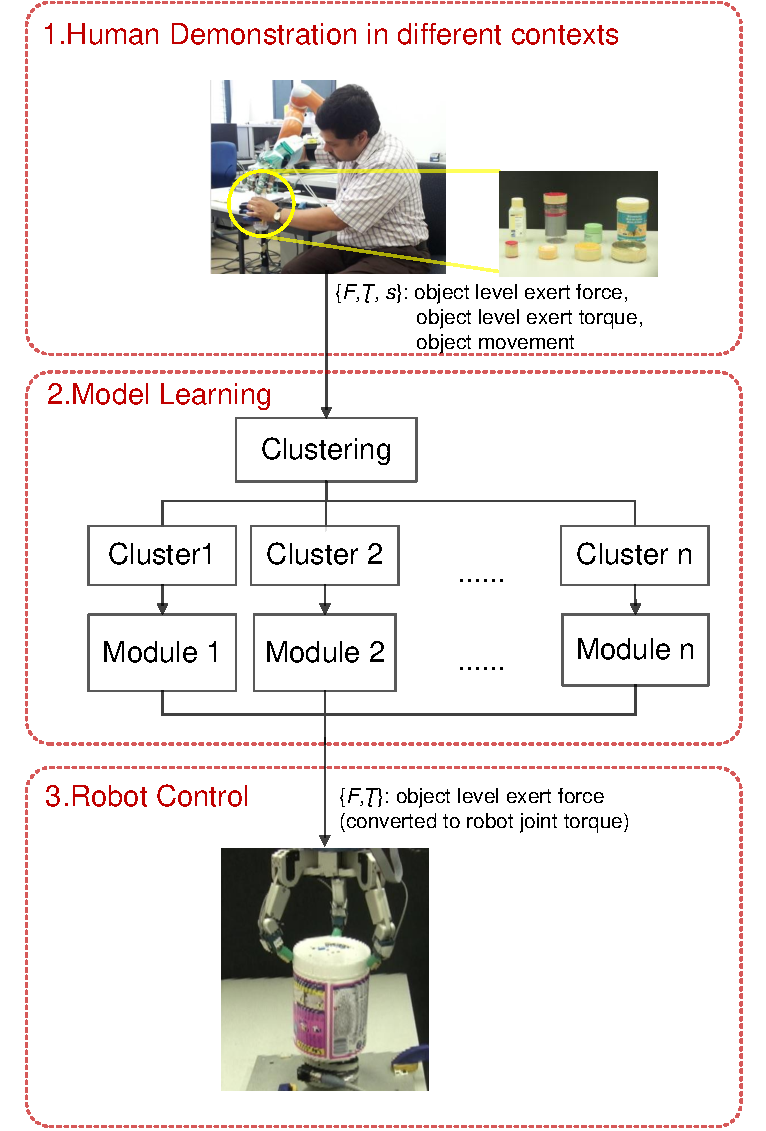
\includegraphics[width=8cm]{./fig/overview5.pdf}
   \caption{ \scriptsize{System overview. Our system takes a
       three-step approach. 1) A human demonstrates a task in a
       variety of contexts. In the opening-bottle-cap experiment, the
       demonstrations are done with different bottles and caps. The
       object-level exerted forces and torque, and the the object's
       movements are used for training. 2) Clustering via machine
       learning is run over the data from the human control
       strategies. Each cluster is then modeled as one module. 3) The
       multiple modules are integrated to compute motor commands to
       control a robot performing the same task in similar contexts.}  }
\label{fig:overview}
\end{figure}

\subsection{Human demonstration}
\label{sec:demo}

%\begin{figure}
%  \centering
%   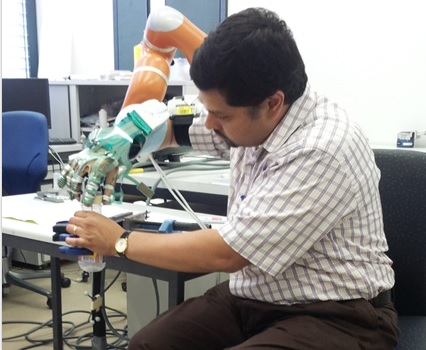
\includegraphics[width=5cm]{./fig/ravin.jpg}
%  \caption{ \scriptsize{Human demonstration of opening a bottle cap.}
%}
%\label{fig:demo}
%\end{figure}

\begin{figure}
  \centering
    \subfloat[\scriptsize{Optitrack markers attaching to a cap}] {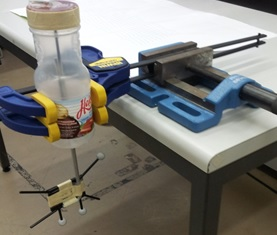
\includegraphics[height=2cm]{./fig/marker2.jpg}}
    \subfloat[\scriptsize{Force torque sensor}] {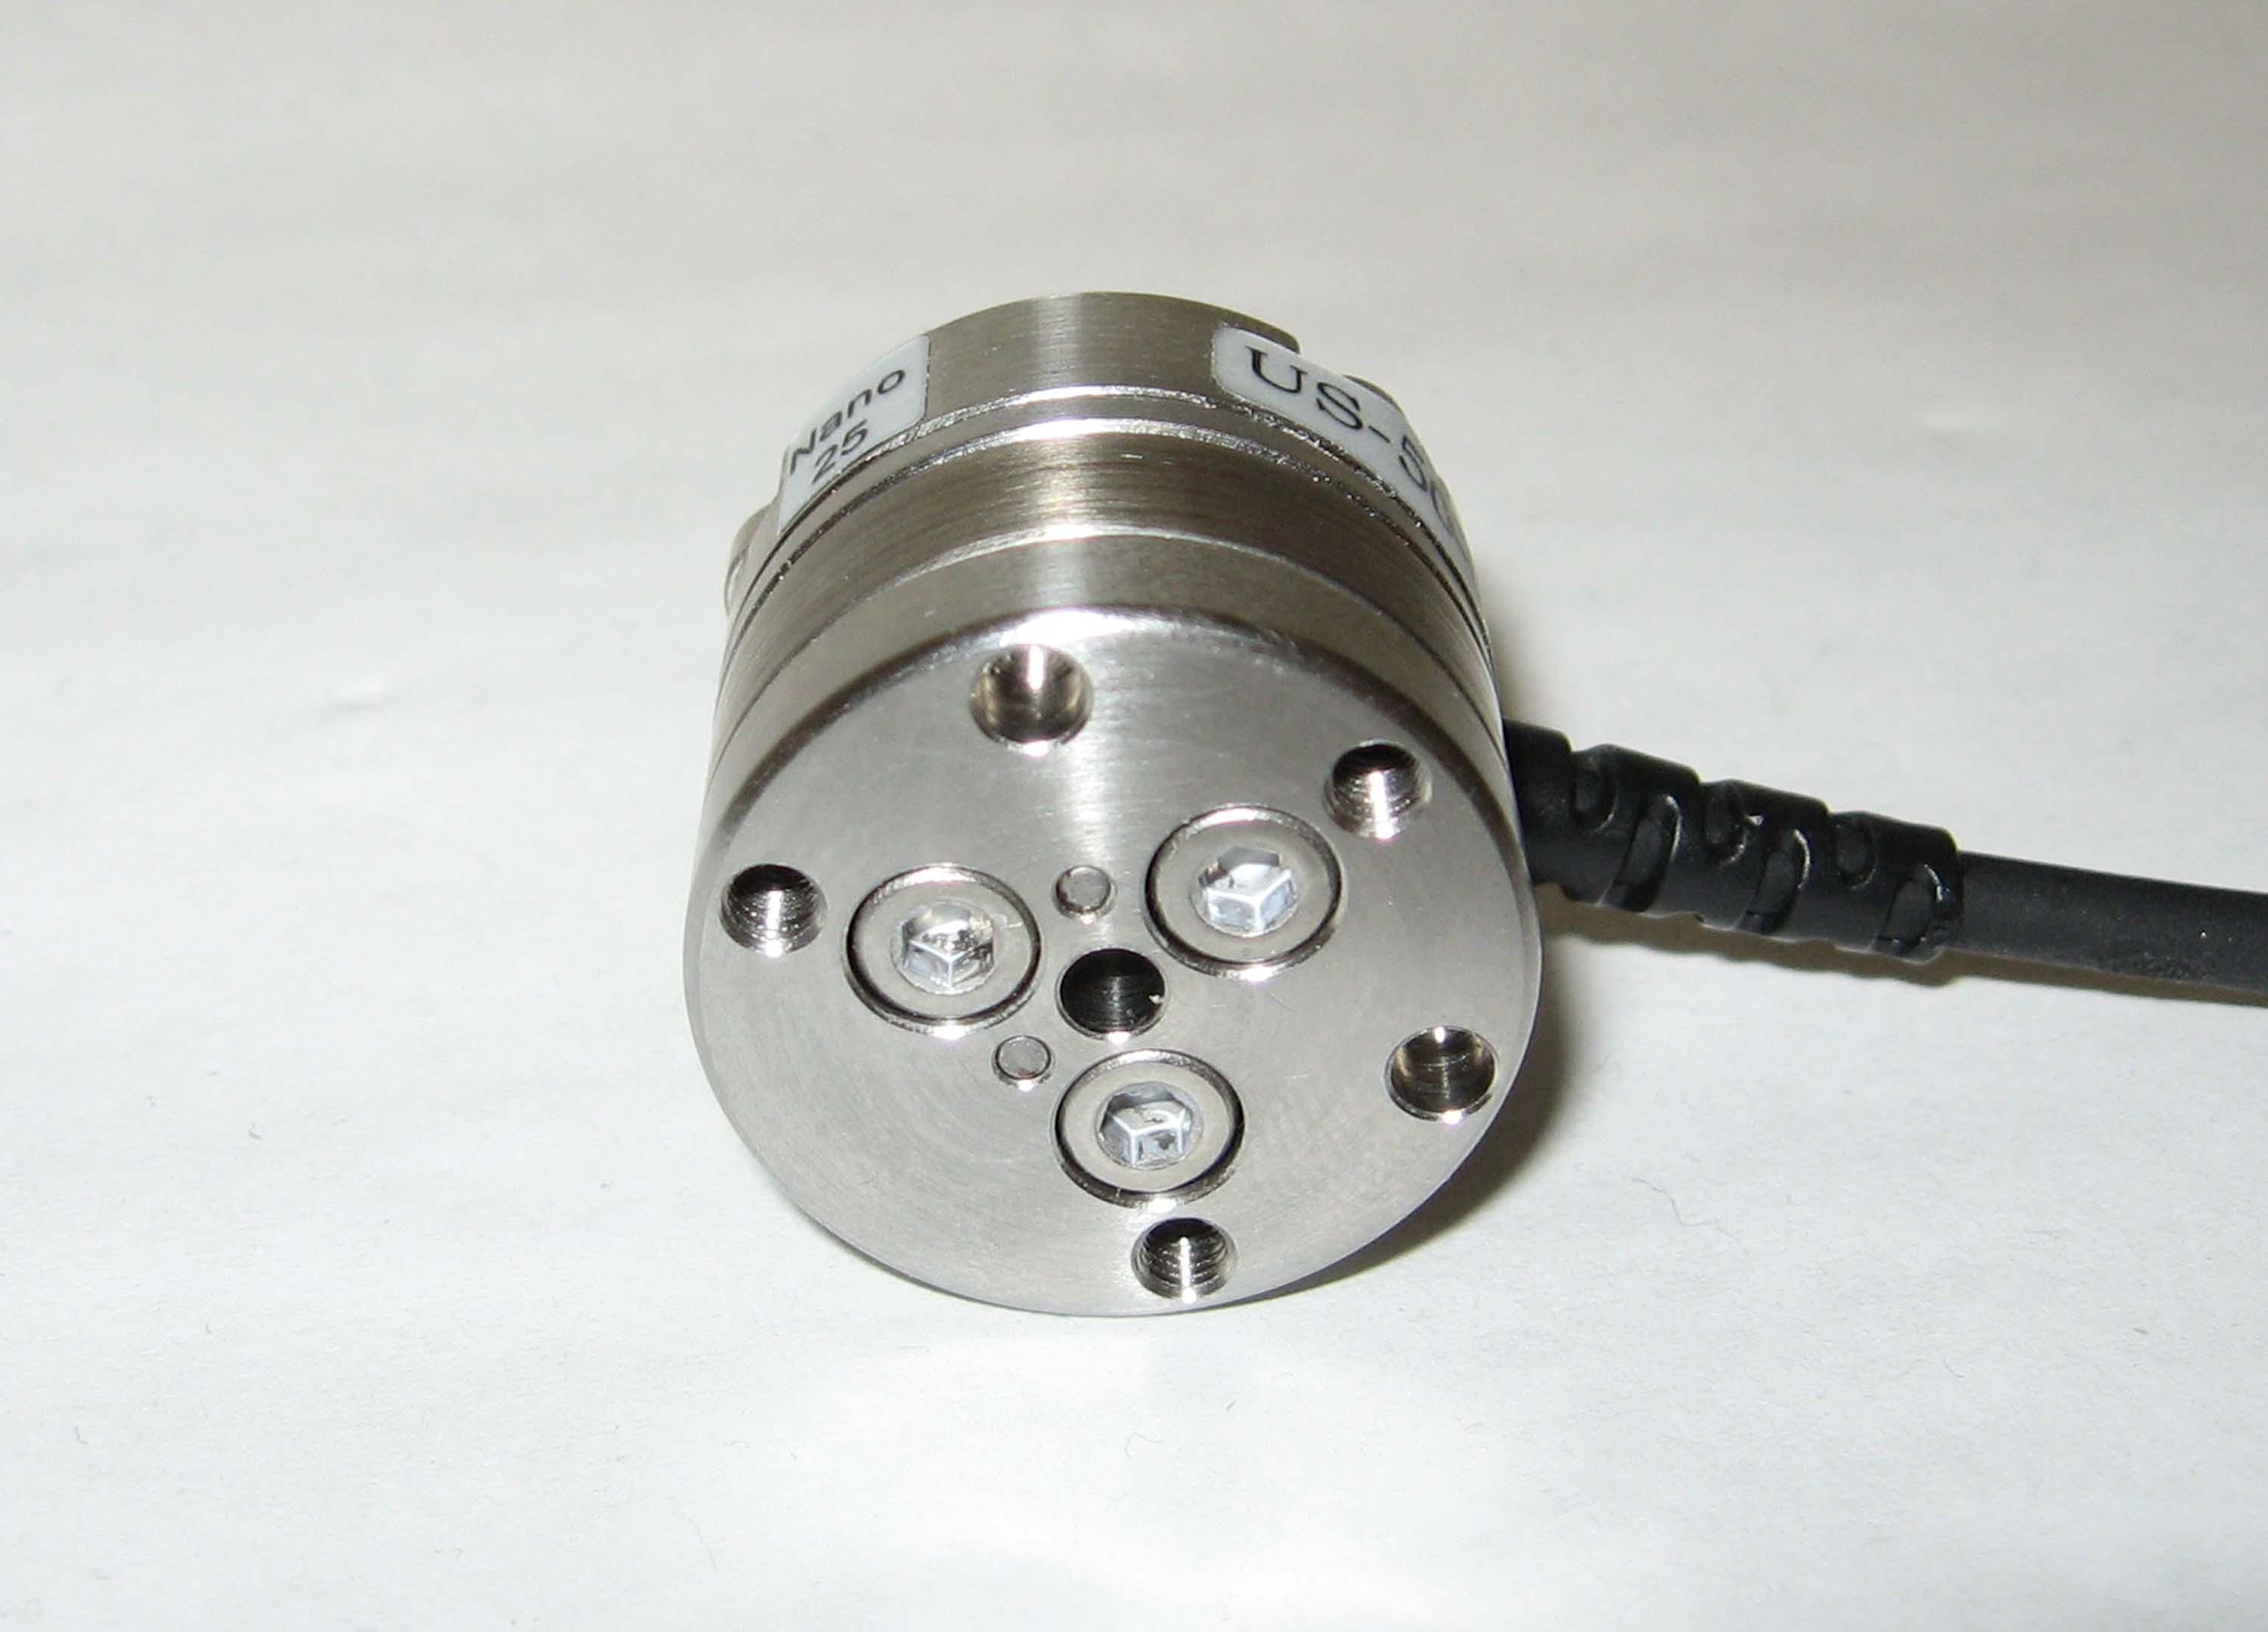
\includegraphics[height=2cm]{./fig/Nano25-E.jpg}}
    \subfloat[\scriptsize{Texscan tactile sensors mounted on a glove}] {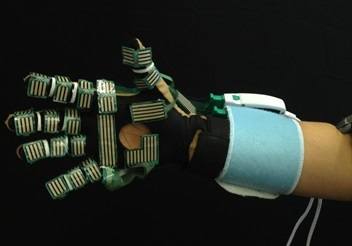
\includegraphics[height=2cm]{./fig/texscan2.jpg}}
    \caption{\scriptsize{Sensors used in the human demonstration of
        opening a bottle cap task.} FIXME why are you using scriptsize
      in the captions?  Is this the latex format from the journal?  Is
      it just so you don't have to increase the size of the text in
      the figures?  Also, should we provide full references for the
      exact sensors we used?  E.g. like this
      \citep{NetLogo2.1,unreal}.}
  \label{fig:devices}
\end{figure}

The first step is recording the human demonstrations of a task. Based on
the object-centric principle, we collect the object's trajectory and its
driving force. % FIXME driving force?  what is the correct term?  Look
              % in articles you read!
We collected this data by a vision-based motion-capture system,
force-torque sensor and wearable haptic
devices. Figure.~\ref{fig:devices} shows a few of the sensors we used
in the opening-bottle-caps task. % JJB this is that section! Details will be explained in
%section~\ref{sec:exp_demo}.

% ===== Why not kinematics approach? =====
%For manipulation task, kinematics teaching on robot is difficult. While a manipulation task usually involves multifinger movement, a human can kinematically operate one finger with each hand and hence two fingers simultaneously for the most extend. Tele-operation of the robot hand solves this problem but it does not provide a direct force feedback. In our approach, human perform the task with direct interaction with the object. With direct interaction with the object the demonstrator is able to perform the task most naturally and perform a more delicate control strategy. %In an object centric manner there is no difference between collecting data from the demonstrator or from the learner -- they are expressed from the objects' perspective. Once the control policy is encoded, it can be directly applied to the robots.

%Kinematics teaching of the learner is not necessary here for three reasons. Firstly in an object centric manner there is no difference between collecting data from the demonstrator or from the learner -- they are expressed from the object point of view. Secondly with direct interaction with the object the demonstrator is able to perform the task most naturally and hence provide a more naturally control policy. Thirdly manipulation with multifinger is difficult to demonstration kinematically, as a human can manipulate one finger of a robot with each hand and hence two fingers simultaneously for its most extend.

% ======= demonstrate in different context   =======
In the demonstrations, the demonstrator performs a task a number of
times to generate enough data to reliably capture its key features.
We determined this level by trial-and-error, in the end using fairly
few trials The demonstrator also performs the task under a variety of
conditions, e.g. a range of friction conditions, in order to explore
how humans adapt to different task contexts.   These different
configurations must be chosen to cover a wide range.% of different
%contexts.  JJB -- redundant.
For example, in a opening-bottle-cap task, the demonstration of opening
the tightest bottle within the capability of the learner is
included. These wide range demonstrations are then used to learn a
multiple module model. Details including the exact numbers and
durations of our trials are described in
Section~\ref{sec:exp_demo}. %FIXME check this is detailed there!

%The force and torque applied on the cap are measured by the Trkscan pressure sensor and a force torque sensor. The movement of the object is recorded by the OptTrack motion tracking system. Each demonstration is recorded as a temporal sequence.

%~\citep{bidan2013robio}
%~\citep{huang2013learning}
%~\citep{huanghumanoid}

\subsection{Learning a Multiple-Module Model}
\label{sec:learn}
Here we detail our modeling method, explaining how we model the human
manipulation strategy.  This requires determining the number of modules to
represent a task strategy, determining the models for driving each
module, and determining how to integrate the output of the modules.

\subsubsection{Object centric manipulation strategy}
\label{sec:objectlevel}
As mentioned in Section~\ref{sec:related}, one of the challenges in
imitation learning is the correspondence problem, i.e. how to map the
demonstrator's motions to the robot's motions so that they produce the
same effects, such as reaching the same
point. %This problem is particularly important in the motion planning tasks.
In an object manipulation task, the goal is to deliver the object from
the current state to a desired state. During this process the movement
of the manipulator is bounded by the movement of the object. Thus it is
more important to imitate how the human applies force to achieve object's
desired movement, than to imitate human limb movement.  This is part
of what justifies our object-centric representational approach.
%Therefore we take an ``object centric approach"~\citep{okamura2000overview}, of which the control policy is taken from the object point of view.

%JJB don't start paragraphs with things like "Therefore", that's
%usually better within paragraphs for connections. The first sentence
%of a paragraph should be strong, self-contained  topic sentence.
The object-centric approach means that our model encodes a force and
torque profile rather than the end effector movement trajectory.  The
imitation-learning objective here is not to find a policy for the end
effector movement but to find a policy that maps  force and torque
to object movements. This policy allows the robot to efficiently
acquire new behaviors to accomplish the
task. %Different robots move differently to achieve the desired object movements.
Giving the robots' kinematics and the desired exerted force and torque
on the object, the robot joint torques can be deduced by their Jacobian
matrix~\citep{okamura2000overview}. To this end, we focus on the
force-torque-displacement tuple: $\{F,\tau,s\}$ demonstrated in the
task, where $F$ is the exerted force in all directions including the
grip force, $\tau$ is the exerted torque in all directions and $s$ is
the object displacement. In later sections, we refer $\{F,\tau\}$ as
the motor command (action) with notation $\{a\}$. In each
demonstration, a time series of the tuple is recorded.



\subsubsection{Deciding the number of modules}
\label{sec:cluster}

% ----------- why clustering -----------
Due to physical interactions with an object, a manipulation task
frequently encounters abrupt changes of the system dynamics, for
example transfer between statuses with no contact and with contact,
between statuses driven by static friction and by driving %FIXME?
dynamic friction. Different strategies should be used to handle
different dynamics.  This motivates our multiple-module
representation. Our approach is to extract strategies from a
demonstration and build one module for each of the
strategies. %During implementation, the system quickly estimate the context by the sensory inputs and choose the most appropriate module or weight and combine the modules to react.

%In this multiple model approach, each model is trained for a particular dynamics context. During the control process the model can compute appropriate control commands for the corresponding dynamics according to the sensory inputs. If the model is chosen properly (see Section~\ref{rf} for mixing model), this approach will be able to adapt to changing environmental context.

% ---------- Cluster to find number of modules -----------
Different tasks may need different number of modules. In the human
demonstrations, the same task is demonstrated with a few different
setups to explore how human adapt to them. However, the number of
setups does not necessary equal to the number of modules needed in the
task. Humans may regard different setups as the same task context and
handle them with the same control
strategies. %Some data may seems to be dissimilar in the scale or frequency, but in fact are governed by the same dynamic.
In order to find a proper number of modules, we need to differentiate
different types of strategies. The differences can be reflected in
different patterns of the force-torque-displacement tuple. We
differentiate the patterns in a data-driven manner: clustering across
the force-torque-displacement tuple. Data in the same cluster is
considered to be governed by the same strategy. The number of clusters
determines the number of modules, and each module is encoded by one model.


% ----------- Distance Metric for clustering ------------
The goal of clustering is to separate a set of data into a few groups
according to their similarities. The first step of clustering is to
measure the similarities, i.e. the distances, between different data
points. Unlike most clustering problems, the data we need to cluster
are not a set of single data points but a set of time series. Here we
use the Dynamic Time Warping technique (DTW) to measure the distance
between each pair of time series~\citep{berndt1994using}.

Dynamic time warping is suitable for measuring the similarity between
two time series, which may have different speeds or durations. It
warps the data in the time dimension and finds the optimal match
between the time series. The similarity is computed as the average
distance between the corresponding points in two series.

The similarity (distance) between each pair of time series is computed
by DTW and produces a distance matrix. In this distance matrix, each
element contains a measurement of the similarity between two time
series. We then cluster these time series into a few groups by a
threshold of the similarity. This threshold is set by using the
variance of the data from the same setup as a reference. As mentioned
above, under the same setup a task is demonstrated a few times. These
demonstrations are presumed to be handled with the same strategy and
hence belong to the same cluster. The variance of these demonstrations
give a reference of a proper variance of a cluster. The largest
variance, across the variance of all setups, is used as the threshold
for the clustering.  %FIXME is this right?  Surely we had different
                     %clusters for different phases of a task within
                     %the same context, and spent some time fixing the segmentation.

%% ------------ Hierarchical clustering -----------
Many of the clustering methods require the specification of the number
of clusters. In our case, however, the number of clusters is an
unknown variable. Therefore we use the hierarchical agglomerative
clustering method~\citep{willett1988recent} to group our
data. Agglomerative clustering is a method that merges similar data
iteratively until the stop criteria is satisfied --- this does not
require a predefined number of clusters. Our clustering method is
described as follow:

\begin{enumerate}
\item At the beginning, each single time series is considered to be one cluster.
\item Compute the distances between each pair of clusters.
\item Starting from the first cluster, find its nearest cluster. We
  define the distance between two clusters to be the average distance
  across all the time series pairs in each cluster. If the distance to the
  nearest cluster is smaller than the threshold, merge these two
  cluster. FIXME  The first time, when there is only one item in each
  cluster\ldots %FIXME explain what happens.  If a two clusters are
                %arbitrarily paired that are far apart (say one is a
                %severe outlier), they will set a very high average
                %with this method.
\item Move to the next cluster. Repeat the last step for the rest of the clusters.
\item A new set of clusters will have been formed by the last few
  steps.  Move to the next step of the hierarchy and repeat the step 2
  to 4 until no new clusters can be formed.
\end{enumerate}

Pseudocode of the complete algorithm is shown in
Algorithm~\ref{code:cluster}.  FIXME this algorithm should include a
line about how the clustering
threshold is computed.  Normally algorithms are {\em more} detailed
than the text description, not less. %FIXME 

\begin{algorithm}
  \caption{Agglomerative Hierarchical Clustering}
  \begin{algorithmic}[1]
%    \Require{$x$ and $y$ are packed strings of equal length $n$}
%    \Statex Init();
    \State Init(): Make each time series a cluster\;
    \State $mergeable$ = true\;
    \Function{Merge}{all clusters, distance matrix} %      \Comment{$\oplus$: bit}
    \While{mergeable is true}
      \State $mergeable$ = false\;
      \For{each cluster}
        \State $ClusterA$ = current cluster\;
        \State $ClusterB$ = nearest neighbor of $ClusterA$\;
        \If{distance($ClusterA, ClusterB$) $<$ clustering threshold}
            \State Merge $ClusterB$ into $ClusterA$\;
            \State $mergeable$ = true\;
        \EndIf
      \EndFor
      %\State \Return{$\delta$}
    \EndWhile
    \EndFunction
  \end{algorithmic}
  \label{code:cluster}
\end{algorithm}



% --------- Number of cluster -----------
When the clusters cannot be merged further, we define the number of
modules for this task: it is the number of the remaining
clusters. Each cluster is used as a module. The pattern of the data in
a cluster represents a strategy for handling a specific task context.

\subsubsection{Learning Models for Modules}
\label{sec:model}
After identifying the number of modules and the data assigned to each,
we build models for each module from its associated data. In this
section, we explain the way we encode human manipulation strategy
using machine learning to build the modules.

During demonstrations, we constantly acquire the object displacements
and the force and torque applied by the demonstrator. The demonstrator
is the only source of exerted force and torque in the system. The
relationship between the exerted force and torque and their resulting
object displacement shows the dynamic characteristics of the task.

%GMM
We model the correlation of the force and the displacement with
GMM. The task dynamics is hence encoded as a joint distribution of the
object status displacement $s$ and the action $a$ taken by the human,
$p(s,a,{\mid}{\Omega})$. In our experiment, $s$ is the one-dimensional
angular displacement of the cap, and $a$ is the one-dimensional
exerted torque and grip force (Section~\ref{sec:exp}).  Modeling their
distribution by GMM allows us to capture the nonlinearity in the data,
and also to compute the likelihood of a query data point in the
model. This provides a good estimation of the reliability of the
module in the current task context, which is crucial in choosing the
correct modules for control (discussed in
Section~\ref{sec:rf}). Further, as a generative model GMM is able to
generate new data from the model, that is it allows us to generate
motor commands. This is done by the {\em Gaussian Mixture Regression}
(GMR). Table~\ref{tab:GMM} explains the encoding process of GMM and
the generative process of GMR.  %FIXME (but maybe not right now) this
% isn't really a table at all, it's a box (but not the kind of box
% latex calls a box).  You can make a new type of float with the float
% package so it doesn't say "Table" on it, but that's probably not
% critical right now -- the publisher will likely fix it.


\begin{table}
    \colorbox{light-gray}{
        \begin{minipage}[t]{0.45\textwidth}

          With a Gaussian Mixture Model (GMM), the joint distribution
          $\Omega$ of a set of variables $\{\eta\}$ is expressed as a
          sum of $N$ Gaussian components:
           \begin{equation}
           \begin{split}
            p\left(\eta\mid\Omega\right) = \sum_{n=1}^N \pi_n p\left(\eta\mid\mu_n,\Sigma_n\right) \\
            = \sum_{n=1}^N \pi_n \frac{1}{\sqrt{\left(2\pi\right)^D \mid\Sigma_n\mid }} e^{-\frac{1}{2}\left(\eta-\mu_n\right)^{\top} \Sigma^{-1}_n \left(\eta-\mu_n\right)}
           \end{split}
           \end{equation}
           where $\pi_n$ is the prior of the $n^{th}$ Gaussian component
           and the ${\mu}_n$, ${\Sigma}_n$ the corresponding mean and
           covariance, and $D$ the number of variables.


            %% GMR:
            Gaussian Mixture Regression (GMR) allows us to estimate the conditional expectation value of a variable $\eta^e$ given a query point $\eta^q$ where $\{\eta\} = \{\eta^q, \eta^e\}$. To compute this expectation value, first we define:
            \begin{equation}
            {
             {\mu}_{n} = \begin{pmatrix} {\mu}_{n}^q    \\
                                         {\mu}_{n}^e
                         \end{pmatrix}
            }
%            \end{equation}
%            \begin{equation}
            \hspace{1cm}
            {
            {\Sigma}_{n} =  \begin{pmatrix} {\Sigma}_{n}^{qq}  & {\Sigma}_{n}^{qe}  \\
                                            {\Sigma}_{n}^{eq} & {\Sigma}_{n}^{ee}
                            \end{pmatrix}
            }
            \end{equation}

            Secondly we compute the expected distribution of $\eta^e$ from the $n-th$ component:

            \begin{equation}
            {
            \hat{\mu}_{n} = {\mu}_{n}^e + \Sigma_{n}^{eq}({\Sigma}_{n}^{qq})^{-1}(\eta^q-{\mu}_{n}^e)
            }
            \end{equation}

            \begin{equation}
            {
            \hat{\Sigma}_{n} = {\Sigma}_{n}^{ee} - {\Sigma}_{n}^eq({\Sigma}_{n}^{qq})^{-1}{\Sigma}_{n}^{qe}
            }
            \end{equation}


            Finally, all the $N$ Gaussian components are taken into
            account, and the expectation value of variable $\eta^e$ is
            computed as the mean $\hat{\mu}^e$ with the covariance
            $\hat{\Sigma}^{ee}$: 

            \begin{equation}
            {
            \hat{\mu}^{e} = \sum_{n=1}^N{\beta_n}\hat{\mu}_{n}
            }
%            \end{equation}
%            \begin{equation}
            \hspace{1cm}
            {
            \hat{\Sigma}^{ee} = \sum_{n=1}^N{\beta_n}^2\hat{\Sigma}_{n}
            }
            \end{equation}

FIXME I'm not checking math
            carefully, but I deleted a little n off this last LHS to
            match the expression that introduced this equation, check
            I'm right?  %FIXME

            where
            \begin{equation}
            {
            \beta_n = \frac{\pi_{n}p(q|{\mu}_{n}^q,{\Sigma}_{n}^{qq})}
            {\sum_{n=1}^N{\pi_n}p(q|{\mu}_{n}^q,{\Sigma}_{n}^{qq})}
            }
            \end{equation}

            Note that in a multiple module model, different module may have different number of Gaussian components.
        \end{minipage}
    }
\caption{Encoding process of GMM and computation process of GMR}
\label{tab:GMM}
\end{table}


%The choice of GMM give us three advantages. Firstly, it is good in modeling nonlinear behavior. Secondly, it tolerates noisy of the data in a good extend and give good estimation of the expected values. Thirdly, as a generative model, it allows the computation of the likelihood of a given input data in the model. This provides an easy measurement of the reliability of the module, which is crucial in choosing the correct modules for control (see Section~\ref{sec:rf}).

%We use the Gaussian Mixture Model (GMM)~\citep{cohn1996active} to encode the task dynamics, and get a joint distribution of the object status $s=\{(x^t,v^t)\}^T_{t=1}$ (displacement $x$ and velocity $v$) and the action taken by human ($a=\{f^t,\tau^t\}^T_{t=1}$) $p(s, a, {\mid} {\Omega})$. The choice of GMM give us three advantages. Firstly, it is good in modeling nonlinear behaviour. Secondly, it tolerates noisy of the data in a good extend and give good estimation of the expected values. Thirdly, as a generative model it is flexible of the type of control: we can compute the force and torque from the given displacement and velocity or compute the displacement and velocity from the given force and torque. %According to different tasks, the variables encoded by GMM may be in different format, e.g. for multi-step prediction control we need to model $s$ in the form of $s=\{x^t,x^{t-1},x^{t-2},...,v^t,v^{t-1},v^{t-2},...\}$. See later section~ref{experiment} for details.


%We aim to build a model closely simulates human motor strategy in order to make the best use of the human data. Evidences of neuroscience suggest that human develop internal model for motor control, so as to estimate the outcome of a motor command. The use of internal model speed up the human correction and reaction in motor control. One hypothesis of the internal model is MOSAIC, which is a multiple modular model composed by a couple of pairs of forward model and inverse model. We build our control strategy based on this hypothesis.

%A forward model is held to anticipate the outcome of the motor command, while an inverse model is held to generate motor commands to take the current system state to the next state. The discrepancy between the anticipation of the forward model and the actual feedback is used to correct the motor command generated from the inverse model (Section~\ref{sec:rf}). Figure~\ref{fig:control} shows the basic control flow of a forward-inverse model pair.

%JJB: note: emulates not simulates.  We're not trying to figure out
%exactly how humans control their muscles, skin & bones.
We aim to build a model that closely emulates the human motor strategy
in order to make the best use of the human data. A forward model is
held to anticipate the outcome of the motor command, while an inverse
model is held to generate motor commands to take the system from the
current state to the next state. The discrepancy between the
anticipation of the forward model and the actual feedback is used to
correct the motor commands generated from the inverse model
(Section~\ref{sec:rf}). Figure~\ref{fig:control} shows the basic
control flow of a forward-inverse model pair.

FIXME Both figure should be labelled ``efferent copy'' not ``effective
copy''.  Also, it's very hard to read ``a1l1'' as ``action 1  x
responsibility 1'', the l looks like a pipe or a capital i. Please use
$\lambda$ as you do in the main text. Finally, all the text
in the figure should be the same size.  The integration is one of the
most important bits of information, so that eqaution needs to be
legible.
Actually, to be clear you should have the efferent signal labeled
(maybe in parentheses under ``Motor command'' in the first figure) as
well as its copy.  And why do you say ``reafferance'' instead of ``afferent''?
% FIXME
\begin{figure}
  \centering
      \subfloat[\scriptsize{}]{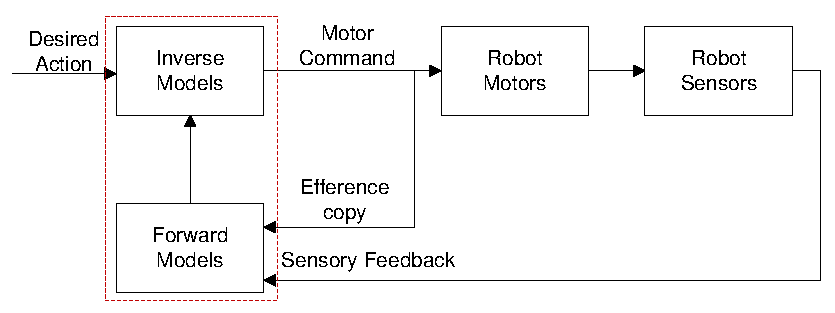
\includegraphics[width=8cm]{./fig/control_1_2.pdf}}
      \vspace{0.5cm}
      \subfloat[\scriptsize{}]{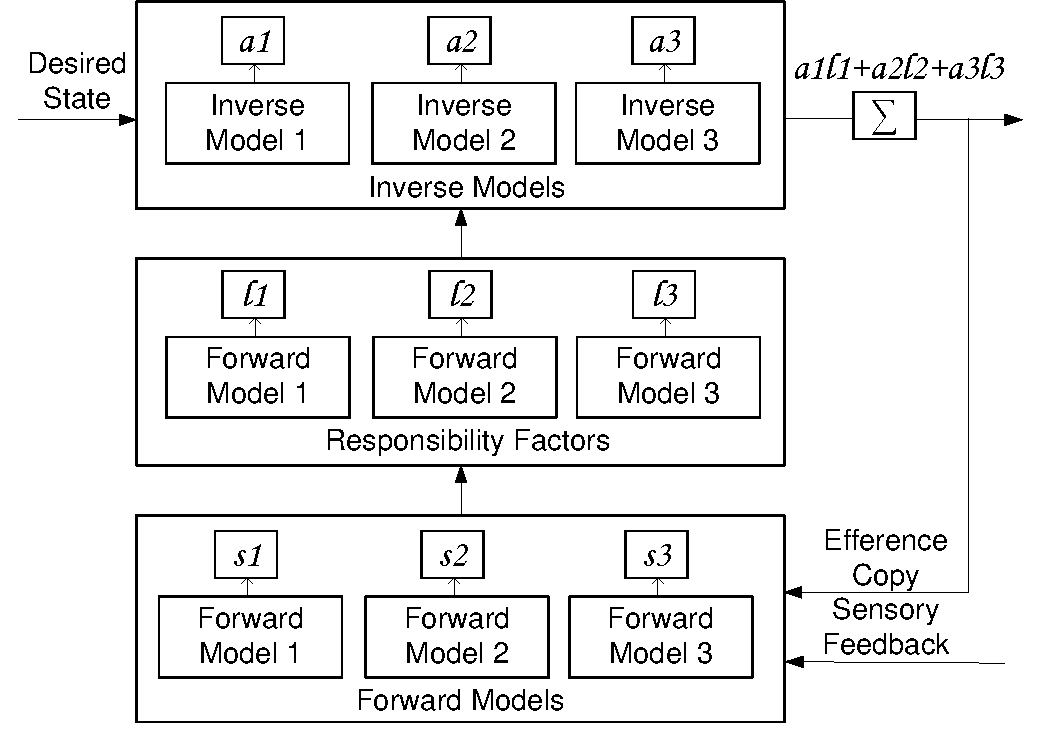
\includegraphics[width=8cm]{./fig/control_3_2.pdf}}
%  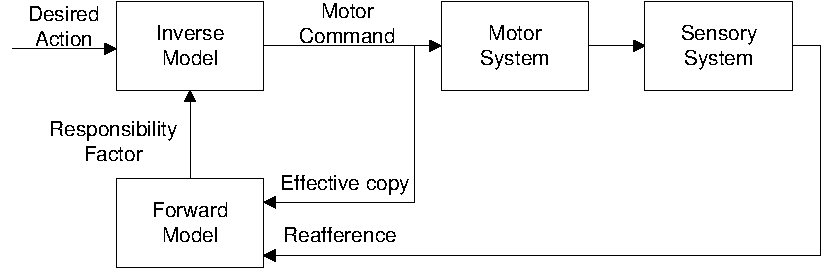
\includegraphics[width=8cm]{./fig/control_1.pdf}
%
%  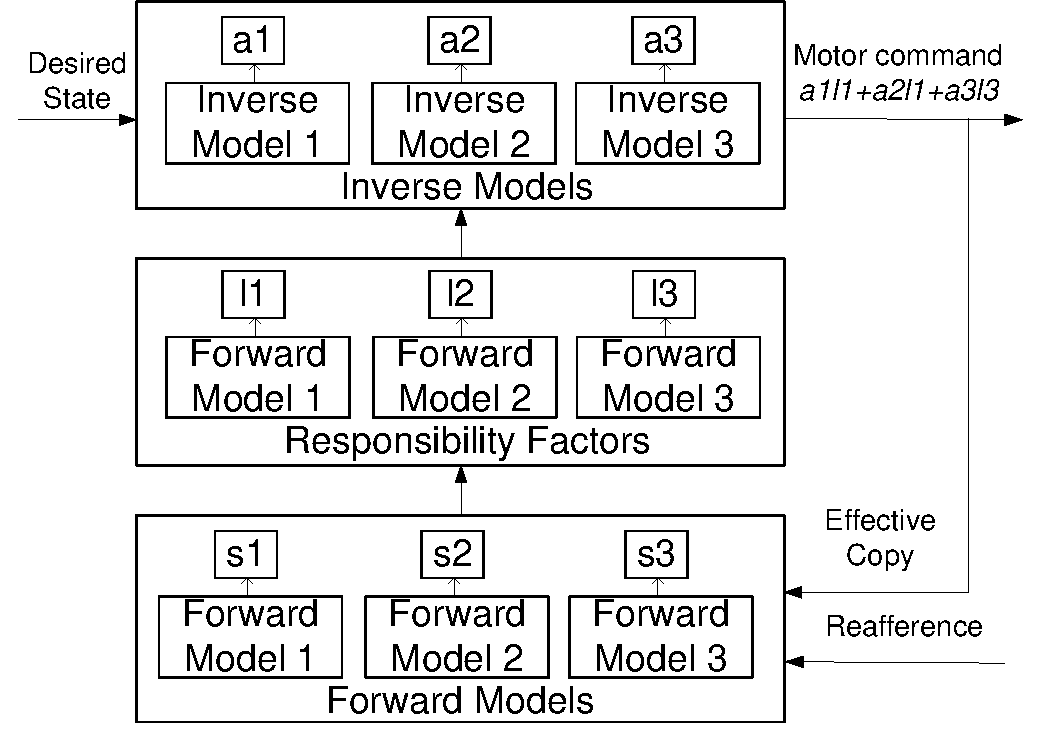
\includegraphics[width=8cm]{./fig/control_4.pdf} %JJB note that
%  there are no final commands in this kind of model, it's continuous.
      \caption{ \scriptsize{Control flow diagram of forward-inverse
          model in motor control. (a) System overview. Pairs of
          forward and inverse models work together to generate motor
          commands. The detailed mechanism inside the red box is shown
          underneath. (b) An example of a 3-module model. The forward
          models predict the current task context (s1, s2, s3) and
          estimate the accuracy of their prediction ($\lambda$1, $\lambda$2,
          $\lambda$3). These accuracy estimates are called ``Responsibility
          Factors'' as they also determine how much responsibility
          each inverse model should take in the final command. The
          inverse models generate commands (a1, a2, a3) and the final
          command is the summation of these, each weighted by its
          individual responsibility factor (a1$\lambda$1+a2$\lambda$2+a3$\lambda$3).  } }
\label{fig:control}
\end{figure}


% --------- one model for each ----------
We encode the forward model $\Omega_F$ by the joint distributions of the current system state (object displacement), previous system state and the previous motor command, i.e. $p(s_t,s_{t-1},a_{t-1}\mid{\Omega_F})$, and similarly encode the inverse model $\Omega_I$ by the joint distributions of the current system state, the desired next system state, previous motor command and the current motor command, i.e. $p(s_t,s^{*}_{t+1},a_{t-1},a_t{\mid}{\Omega_I})$.
%Given the previous system state and motor command, the GMR provides a close-form solution to compute the expected system state $s_t$, i.e. $E(s_t{\mid}s_{t-1},a_{t-1},{\Omega_F})$. 
The previous motor command $a_{t-1}$ is necessary for the inverse
model. In some tasks, the system status can remains unchanged for a
certain period until the exerted force reaches a threshold to change
it. This will cause degeneracy in the inverse model; hence we 
include the previous motor command in the model to tackle it.



% Non-linear, multi model. What to solve in multi model
%As discussed above, one of the characteristics of manipulation task is the changing kinematics and dynamics configuration.
%In different task contexts, the pattern of the correlation between the displacement and action may be different.
%By clustering the training data into different groups (Section~\ref{sec:cluster}), we are able to discover the number of different patterns, i.e. number of modules. We train one GMM on each of the modules to encode the different changing patterns of the task context.


% Learn system dynamics, impedance, admittance.

%Phases
%A single model is usually not enough to encode all these different
%configurations. Therefore we adopt a multiple modular approach to
%model the different environment. 




\subsection{Modular adaptive control and integration}
\label{sec:control}
%% forward-inverse modeling
%%After clustering the data into different groups, we train each cluster with the GMM $p(X_T, X_{t+1}, U_{t-1}, U_t {\mid} {\Omega})$.
%We model each of the cluster to encode the human control policy under different dynamics.
%Neuroscientists suggested that human use a mixture of forward model and inverse model for motor control. The forward model
%With the learned multiple models, we adopt the MOSAIC~\citep{haruno2001mosaic} architecture to control the system. The basic concept of MOSAIC is that the human brain use multiple inverse models to control the system, which is augmented with a forward models. In human brain there exist multiple pairs of coupled forward and inverse models. The forward models estimate the reliability of the inverse model in the current context, and the final motor command is a linear combination of all the commands from the inverse models.
%In object manipulation, the system dynamics can be rapidly changing over time and we need more than one model to describe it. Our learnt multiple GMMs are used to describe the system in these different contents. First we need to infer the behavior of the system. Having deduced this information, we need to decide how to manipulate the system.

Once the number of modules is found and a pair of forward and inverse
models has been learnt for each, the modules can be used to compute
motor commands for task execution.  In our system of action selection,
this process of computing the command also computes a weight which
allows integration of the modules by simple summation.  We consider
the human motor system acted upon by motor command $a_t$ at time $t$
with current system status $s_t$. A function $f$ maps $a_t$ and $s_t$
to the system status at time $t+1$:
\begin{equation}
\label{e1}
s_{t+1} = f\left(s_t,a_t\right)
\end{equation}
The goal of the controller is to generate a motor command $a_t$ that
brings the current system status from $s_t$ to a desired state $s^*_{t+1}$:
\begin{equation}
\label{e2}
a_t = g\left({s^*_{t+1},s_t}\right)
\end{equation}

Equation~\ref{e1} represents the forward model and Equation~\ref{e2} represents the inverse model. In the modular approach, it takes two steps to compute the motor command $a_t$:
\begin{enumerate}
\item Anticipate the sensory output and compute the responsibility factor $\lambda_t$.
\item Compute motor command by each inverse model and compute the final motor command $a_t$.
\end{enumerate}


%\subsubsection{Anticipate sensory output by forward model}
%\label{sec:forward}
%With the $k$-th forward model we can estimate the current state ${\hat{s}} ^k_t$ by the $GMR$ (Table~\ref{tab:GMM}):
%\begin{equation}
%\label{e3}
%{\hat{s}} ^k_{t} = E\left({s_t {\mid} s_{t-1}, a_{t-1}, \Omega^k_I}\right)
%\end{equation}
%
%This equation is to predict the environment status based on the observation and the knowledge of the $k$-th module. In the next step, the prediction will be compared to the actual sensory feedback. The accuracy of this prediction will decide the weight of each inverse model.

\subsubsection{Responsibility factor}
\label{sec:rf}

In a modular approach, choosing the proper modules to control the
system at every time increment is a crucial step. For this we rely on
a system of {\em responsibility factors}, which act as the weights of
the inverse models. The responsibility factor is a measurement of the
reliability of using one module to represent the current system
context.

%The measurement is computed by the discrepancy between the anticipating current system state $s_t$ of the forward model and the actual current system state $s'_t$ from the sensory feedback:
%
%\begin{equation}
%\lambda'^j_t = {$s'_t$ - p(s_t{\mid}s_{t-1},a_{t-1},\Omega^j)}}
%\end{equation}
%
%where $n$ is the number of models.

With the $k^{th}$ forward model we can anticipate the current state ${\hat{s}} ^k_t$ by using $GMR$ (Table~\ref{tab:GMM}):
\begin{equation}
\label{e3}
{\hat{s}} ^k_{t} = E\left({s_t {\mid} s_{t-1}, a_{t-1}, \Omega^k_I}\right)
\end{equation}

By comparing the anticipated current state ${\hat{s}} ^k_t$ with the
actual current state $s_t$ detected by the sensors, we can evaluate
how well the $k^{th}$ module represents the current system. The actual
current state, previous state and the previous motor command form a
data point $\eta_t$ = $\{s_t,s_{t-1},a_{t-1}\}$. As the forward models
are built as GMM, it is easy to compute the likelihood of one data
point belongs to a particular model: $p(\eta_t {\mid}
\Omega_F^j)$. The discrepancy between $\hat{s}^k_t$ and $s_t$ is
embedded in this likelihood and hence in practice we only compute the
$p(\eta_t {\mid} \Omega_F^j)$ and skip ${\hat{s}} ^k_t$.  The
responsibility factor of the $k^{th}$ inverse model is the likelihood of
the data point $\eta_t$ belongs to the $k^{th}$ module, normalized by
the total sum:

\begin{equation}
\lambda^j_t = \frac{p(\eta_t {\mid} \Omega_F^j)}{\sum_{k=1}^{K}{p(\eta_t {\mid} \Omega_F^k)}}
\end{equation}
where $K$ is the number of modules~\footnote{In the case that the
  dominator is very close to zero, the whole control process will be
  terminated as it indicates that the model is used on a different
  task.}.  At every time step, we compute the responsibility factor
for each module. The final motor command at that time step is the
linear combination of the commands generated from each inverse model
multiplied by its respective responsibility factor.

%Note the forward model is embedded in this computation of the responsibility factor. The likelihood of the query point $p(s_t,s_{t-1},a_{t-1}\mid \Omega^j$ in the $j-th$ module is equivalent to the discrepancy between the expected current system state $s_t$ of the forward model and the actual current system state $s'_t$ from the sensory feedback, factorized by the variance of the forward model.

\subsubsection{Generating motor commands by inverse models}
\label{sec:inverse}
%While the forward models predict the current status of the system by the previous status and motor commands, the inverse models generate the next motor command according to the current status and the next target status. In reality, given a current state and a desired state, the command bring the robot to the desired state is not unique. In addition, during object manipulation, it is often the case that the force applying on the object various but the object position does not change because of friction. Therefore we include the previous command into the query point in order to generate the next command without redundance. Hence the command generated by each model is computed by equation~\ref{e4}.
%\subsubsection{Mix of Model}
%\label{mix}

The motor command $a^k_t$ for the $k^{th}$ inverse model is computed
by GMR with the steps explained in Table~\ref{tab:GMM}. At each time
step, the responsibility factors $\lambda^k_t$ weight its
corresponding inverse model: the higher the responsibility is, the
more responsibility the inverse model takes in the control. The final
motor command generated by this multiple model system is:

\begin{equation}
\label{e_mix}
a_t = \sum_{k=1}^K{\lambda_t^k a_t^k} = \sum_{k=1}^K{\lambda_t^k E\left({a_t \mid s^*_{t+1},s_t, a_{t-1}, \Omega^k_I}\right)}
\end{equation}

These three steps are all computed with a close form solution. This ensures that this system can react quickly to the changes in the environment by adjusting the responsibility factor.



